\documentclass[12pt]{article}
\usepackage[utf8]{inputenc}
\usepackage[english]{babel}
\usepackage[]{amsthm} %lets us use \begin{proof}
\usepackage[]{amssymb} %gives us the character \varnothing
\usepackage[margin=1in]{geometry}
\usepackage[shortlabels]{enumitem}
\usepackage{xcolor}
\usepackage{graphicx}
\usepackage{hyperref}

\newtheorem{theorem}{Theorem}[section]
\newtheorem{corollary}{Corollary}[theorem]
\newtheorem{lemma}[theorem]{Lemma}
\newtheorem{definition}[theorem]{Definition} 
\newtheorem{exercise}{Exercise}
\newtheorem{subexercise}{Exercise}[exercise]
 
\newcommand{\R}{\mathbb{R}}
\newcommand{\Q}{\mathbb{Q}}
\newcommand{\N}{\mathbb{N}}
\newcommand{\F}{\mathbb{F}}
\newcommand{\e}{\epsilon}

\renewcommand\qedsymbol{$\blacksquare$}
 
\title{MIRI: Topological Fixed Points}
\author{OS}

\begin{document}
\maketitle


\subsection*{Exercises}


\begin{exercise}
    (1-D Sperner's lemma) Consider a path built out of $n$ edges. Color each vertex blue or green such that the leftmost vertex is blue and the rightmost vertex is green. Show that an odd number of the edges will be bichromatic.
\end{exercise}

\begin{figure}[h]
    \centering
    
\includegraphics[width=15cm]{Fixed_points_1.png}
    
    \label{fig:my_label}
\end{figure}


\begin{proof}

    \begin{itemize}
        \item We claim the Corollary that if the ends of the chain are the same color then an even number of the edges are bichromatic.
        \item Any chain of length $(n+1)$ can be constructed from a sub-chain of length $n$ and then adding the required final vertex.
        \item Suppose both the Lemma and its Corollary hold for a chain of length $n$.
        \item If the sub-chain has matching ends (and even bichromatic edges) then a new vertex must be added of a different colour to get mismatched ends. Then a single bichromatic edge is added, resulting in an odd number of bichromatic edges.
        \item If the sub-chain has mismatched ends (and odd bichromatic edges) then a new vertex must be added to the same color (adding no brichomatic edges).
        \item Therefore the final chain of length ($n+1$) will have odd bichromatic edges.
        \item The Lemme and Corollary hold for $n = 2$ vertices, so the proof follows by induction.
    \end{itemize}

\end{proof}


\begin{exercise}
    (Intermediate value theorem) The Bolzano-Weierstrass theorem states that any bounded sequence in $\R^n$ has a convergent subsequence. The intermediate value theorem states that if you have a continuous function $f:[0,1] \to \R$ such that $f(0)\leq0$ and $f(1) \geq 0$, then there exists an $x \in [0,1]$ such that $f(x)=0$.
    
    Prove the intermediate value theorem. It may be helpful later on if your proof uses 1-D Sperner's lemma and the Bolzano-Weierstrass theorem.
\end{exercise}

With BW theorem. It's a little convoluted. I've added a slightly improved version afterwards that doesn't use BW but does exploit the compactness of the sets:

\begin{proof}

    \begin{itemize}
        \item Firstly define any interval $[a,b]$ as ``crossing'' iff $f(a) \leq 0$ and $f(b) \geq 0$ or $f(a) \leq 0$ and $f(b) \geq 0$.
        \item Define a partition $P_n$ of the interval $[0,1]$ as the division of the interval into $n$ evenly spaced closed intervals of length $1/n$ each. (So $P_1 = \{[0,1]\}, P_2 = \{[0,1/2], [1/2,1]\}, \\P_3 = \{[0,1/3],[1/3,2/3], [2/3,1]\}$, etc).
        \item Applying Sperner's 1D lemma directly here, it follows that there is always an odd number of intervals in partition $P_n$ that are ``crossing''. Therefore, there is at least one crossing interval in each partition $P_n$.
        \item Index a sequence $\{x\}$ so that each element of the sequence $x_i$ is the midpoint of the arbitrarily chosen crossing subintervals. 
        \item Note that this sequence is bounded in $[0,1]$. The BW theorem states that there will be some convergent subsequence which converges to some $x^* \in [0,1]$. Call this sequence $\{x'\} = \{x_{s_1}, x_{s_2}, \ldots\}$.
        \item Consider now $f(x^*)$. If $f(x^*)=0$, our result is obtained. Suppose instead $f(x^*)=\epsilon>0$.
        \item By the continuity of $f$, there exists some $\delta > 0$ such that $f([x^*-\delta, x^*+\delta]) \subseteq [f(x^*)-\epsilon/2, f(x^*)+\epsilon/2]$. Therefore $f([x^*-\delta, x^*+\delta]) > 0$.
        \item Choose some $n \in \N$ such that $1/n < \delta/2$. Now select some $s_i$ such that $|x_{s_i} - x^*|<\delta/2$ and $s_i \geq n$.
        \item By construction $x_{s_i}$ is contained in some crossing interval that is nested within $[x^*-\delta, x^*+\delta]$.
        \item Therefore, the map ($f(.)$) of one end point of this interval must to less than or equal to zero, which contradicts our previous result about the image of the interval being strictly positive.
        \item The proof follows analogously for $f(x^*) < 0$.
    \end{itemize}

\end{proof}

Without BW theorem, but using the fact that an infinite intersection of nested compact intervals is non-empty:

\begin{proof}

    \begin{itemize}
        \item Firstly define any interval $[a,b]$ as ``crossing'' iff $f(a) \leq 0$ and $f(b) \geq 0$ or $f(a) \leq 0$ and $f(b) \geq 0$.
        \item Define a partition $P_n$ of the interval $[0,1]$ as the division of the interval into $2^n$ evenly spaced closed intervals of length $1/n$ each. (So $P_0 = \{[0,1]\}, P_1 = \{[0,1/2], [1/2,1]\}, \\P_2 = \{[0,1/4],[1/4,1/2],[1/2,3/4], [3/4,1]\}$, etc).
        \item Define a sequence of nested intervals as follows. Following Sperner's 1D lemma, any crossing interval has at least one crossing subinterval. Beginning at $n=1$, pick the crossing subinterval $S_1$. At the next step, pick the subinterval of this interval that is crossing, and so on. This defines a sequence of nested crossing subintervals $S_n$. Note $S_n = \bigcap_n S_i$
        \item Let $x^* \in S_{\infty} = \bigcap_{\infty} S_i$. Therefore $x^* \in S_n$ for all $n \in \N$.
        \item Suppose $f(x^*)>0$. By continuity, there is some interval $f([x^*-\delta, x^*+\delta]) > 0$.
        \item Choose some $n \in \N$ such that $1/n < 2/\delta$. It follows that $S_n$ is nested within $[x^*-\delta, x^*+\delta]$.
        \item Therefore, the map ($f(.)$) of one end point of $S_n$ must to less than or equal to zero, which contradicts our previous result about the image of the interval being strictly positive.
        \item The proof follows analogously for $f(x^*) < 0$.
    \end{itemize}

\end{proof}

\begin{exercise}
    (1-D Brouwer fixed point theorem) Show that any continuous function $f: [0,1] \to [0,1]$ has a fixed point (i.e. a point $x \in [0,1]$ with $f(x)=x$).
    
    Why is this not true for the open interval $(0,1)$?
    
\end{exercise}

\begin{proof}
    \begin{itemize}
        \item Define $g(x) = x - f(x)$.
        \item It follows that $g(0) \leq 0$ and $g(1) \geq 0$.
        \item By the IVT, it follows that $g(x) = 0$ for some $x$. Therefore $g(x) = x - f(x) = 0 \Rightarrow f(x) = x$.
        \item The open interval does not contain the end points, which would allow for the construction of a function such as $f(x) = 1$, which sits entirely above the diagonal on the $[0,1] \times [0,1]$ square apart from the endpoint.
    \end{itemize}
\end{proof}

\begin{exercise}
    (2-D Sperner's lemma) Consider a triangle built out of $n^2$ smaller triangles as shown. Color each vertex red, blue, or green, such that none of the vertices on the large bottom edge are red, none of the vertices on the large left edge are green, and none of the vertices on the large right edge are blue. Show that an odd number of the small triangles will be trichromatic.
\end{exercise}

\begin{figure}[h]
    \centering
    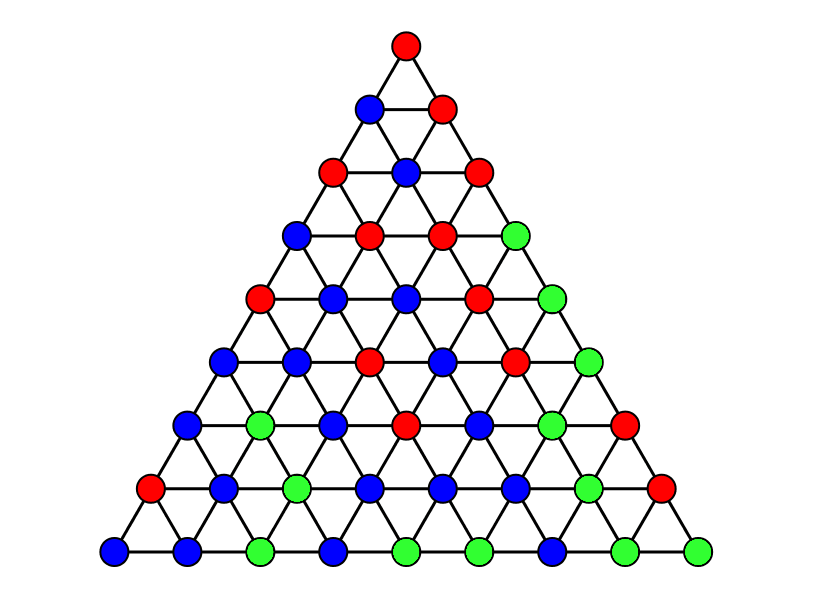
\includegraphics[width=10cm]{fixed_points_2.png}
    \label{fig:my_label}
\end{figure}

\begin{proof}
    \begin{itemize}
        \item Consider some target triangle of sides $n$. This proof proceeds in two parts - firstly that a triangle of that size can be constructed with the required edge conditions fulfilling oddness, and secondly that the internal points can be permuted to get to any target triangle without breaking the oddness criteria.
        \item Suppose we have a triangle of lengths $n$ that fulfills the edge condition and with an odd number of trichromatic triangles. Now add a layer of edges to one of the edges to construct a new triangle of lengths $n+1$. To maintain the edge condition, an edge with the same pair of colours must be matched. Clearly, no trichromatic triangles can be added in this new layer. So the new triangle of lengths $n+1$ will fulfill the oddness criteria. The condition is fulfilled trivially for $n=1$, so the result follows by induction.
        \item Now consider any internal point being changed and consider the hexagon of six triangles it sits in. We will show that changing the internal point will always result in an even number of trichromatic triangles being added or removed.
        \item Consider the $6$ points surrounding that point on the vertices of the hexagon and unwrap it into a sequence of $7$ vertices and $6$ edges with a arbitrary vertex repeating as the first and last. Each trichromatic triangle must be constructed from a set of bicrhomatic edges along this unwrapped perimeter alongside a centre of the missng colour.
        \item We will show that the 3 possible bichromatic edges on this unwrapped sequence (RG, GB, BR) always occur all even or all odd. This means that if the centre changes, we lose an odd number of trichromatic triangles (from one bichromatic configuration) and gain an odd number (from another bichromatic configuration); or we lose an even number and gain an even number. Either way, the net change in bichromatic edges and therefore trichromatic triangles is even.
        \item Take an arbitrary sequence of length $n$ edges and suppose that the condition holds (the three bichromatic edges occur all evenly or all oddly). Then take add any vertex to the inside of the sequence (i.e. not first or last).
        \item Any bichromatic edges that are lost will either be replaced by two of the remaining configurations (i.e. BG $\to$ BR, RG) or be shifted (i.e. BR $\to$ BB, BR). Monochromatic edges will either introduce an even pair (i.e. BB $\to$ BG, GB) or have no change (i.e. BB $\to$ BB, BB). Therefore the full evenness or full oddness is always maintained.
        \item The property clearly holds for $n=1$, so by induction it holds for $n=6$. Therefore, changing the centre point will ``swap'' over odd to odd trichromatic triangles or even to even, resulting in a net even change.
        \item Therefore, for any target triangle, we can construct it by creating the target size with the edge conditions and oddness criteria, then changing internal points. Trichromatic triangles are added or removed in even chunks, so the net effect will always maintain the oddness criteria.
    \end{itemize}
\end{proof}

\begin{exercise}
    Color the all the points in the disk as shown. Let $f$ be a continuous function from a closed triangle to the disk, such that the bottom edge is sent to non-red points, the left edge is sent to non-green points, and the right edge is sent to non-blue points. Show that $f$ sends some point in the triangle to the center.
\end{exercise}

\begin{figure}[h]
    \centering
    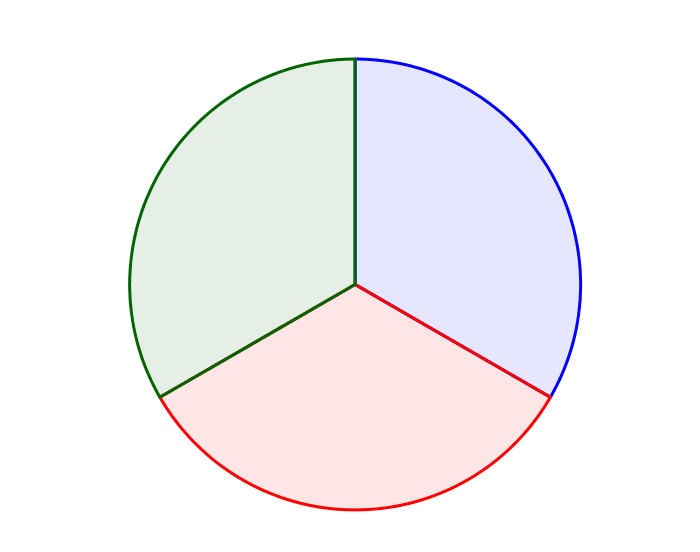
\includegraphics[width=10cm]{fixed_points_3.png}
    \label{fig:my_label}
\end{figure}

\begin{proof}
    \begin{itemize}
        \item This proof proceeds assuming we begin with an equilateral closed triangle of edge length $1$, but can be easily generalised to any other triangle as there exists an isomorphism between the two shapes.
        \item Define a partition $P_n$ of the closed triangle as the division of the triangle into a set of tessellating equal sized equilateral sub triangles such that there of $n$ sub-triangles along each edge (i.e. see Figure 2). The area of each triangle will be $\frac{3}{2n^2}$.
        \item Using Sperner's lemma, there is always at least one trichromatic subtriangle in $P_n$ whose three vertices are in the three sections of the disc (call these $R, G, B$), Construct a sequence $\{x\}$ consisting of the midpoint of an arbitrary trichromatic triangle at each $n$.
        \item Using the BW theorem, there is some subsequence of points that converge. Call this $\{x_s\}$, and its limit is $x_s^*$.
        \item Suppose $f(x^*_s) \neq 0$ but instead say $f(x^*_s) \in R$. By the continuity of $f$, there is some open ball $B(f(x^*_s),\epsilon) \subset R$ and there is some $\delta$ such that $f(B(x^*_s,\delta)) \subseteq B(f(x^*_s),\epsilon)$ for some sufficiently small $\epsilon > 0$.
        \item Choose some $\epsilon$ where $B(f(x^*_s),\epsilon) \subset R$. Then, there is some $\delta$ such that $f(B(x^*_s,\delta)) \subseteq B(f(x^*_s),\epsilon/2)$.
        \item Choose some large enough $x_{s_i} \in \{x\}$ such that $|x_{s_i} - x^*| < \delta$ and $s_i \geq m$ for $1/m < \delta$.
        \item Therefore, $x_{s_i}$ will the midpoint of a triangle that is nested entirely within $(B(x^*_s,\delta)$, and therefore the triangle will map entirely to $R$, which contradicts the construction of the sequence.
    \end{itemize}
\end{proof}

\begin{exercise}
    Show that any continuous function $f$ from closed triangle to itself has a fixed point.
\end{exercise}

This is a pretty straightforward visual proof but quite challenging to (succinctly) describe verbally.

\begin{proof}
    \begin{itemize}
        \item We begin by embedding the triangle $T$ in $R^2$. Let the height of the triangle be $h$ and base $b$. Let the centroid of the triangle be at $(0, 0)$, the upper corner at $(0, h/2)$, the lower left at $(-b/2,-h/2)$, and lower right at $(b/2,-h/2)$.
        \item Define $g(x): f(x)-x$. Note that this maps $T \to \R^2$.
        \item We now note the following: At any point $x$ on the edge of $T$, the function $g$ can only be mapped to a triangular region the same dimensions as $T$, except translated evenly so that $x$ is mapped to $0$.
        \item We can note that the loop generated as the image of the edge of the triangle therefore follows certain restrictions. For example, the image of the bottom edge is restricted have a vertical co-ordinate $\geq 0$, (as the vertical difference is always non-negative). The image of the left edge is restricted to the right hand side of a line through the origin parallel to the left slope, and similarly for the right edge.
        \item Importantly, this ensures that any loop generated must enclose the origin $0$, and three lines can be drawn from the origin that bisect the map of each of the three edges\footnote{Specifically this is always guaranteed for lines from the origin at $0$, $2\pi/3$, and $4\pi/3$, though the proof is tedious} (the map of each edge has a region it uniquely traverses without any other edge's map in that region).
        \item Draw an arbitrarily large circle centred on the origin, with the three arbitrary lines dividing the circle into three segments. In can be checked this fulfills the conditions of the mapping in Exercise 5, so there must exist some point $x^*$ in $T$ such that $h(x^*) = 0$.
        \item Since $h(x^*) = 0$, $f(x^*) - x^* = 0$ and $f(x^*) = x^*$.
    \end{itemize}
\end{proof}

\begin{exercise}
    (2-D Brouwer fixed point theorem) Show that any continuous function from a compact convex subset of $R^2$ to itself has a fixed point. (You may use the fact that given any closed convex subset $S$ of $R^n$, the function from $R^n \to S$ which projects each point to the nearest point in $S$ is well defined and continuous.)
\end{exercise}


\begin{proof}
    \begin{itemize}
        \item Since $S$ is compact we can enclose $S$ in some triangle $T$. Denote $U = T \setminus S$.
        \item Construct a function $g$ as follows. For $x \in T$, $g = f$ where $f$ is the continuous function from $S \to S$. For $x \in U$, $g$ is the continuous function that projects it to the closest point on $S$.
        \item The function is continuous within $T$ (it is continuous on both functions, and the two functions meet at any point on the edge of $S$).
        \item As we have established, a continuous function mapping $T$ to itself must have a fixed point. Since this fixed point cannot be on any point $U$ (as $U$ always maps to $S$ and $S \cap U = \emptyset$), it must lie in $S$.
    \end{itemize}
\end{proof}

\begin{exercise}
    Reflect on how non-constructive all of the above fixed-point findings are. Find a parameterized class of functions where for each $t \in [0,1], f(t): [0,1] \to [0,1]$, and the function $t \to f(t)$ is continuous, but there is no continuous way to pick out a single fixed point from each function (i.e. no continuous function $g$ such that $g(t)$ is a fixed point of $f(t)$ for all $t$).
\end{exercise}


\begin{proof}
    \begin{itemize}
        \item $f(t,x) = \frac{1}{1+e^{t-x}}$
        \item A broad range of sigmoid functions such that:
        \begin{itemize}
            \item $f(0)\in (0,1)$, $f(1) \in (0,1)$
            \item For $x^*$ s.t. $f''(x^*)=0$, $f(x^*) > x*^$ for $t = 0$ and $f(x^*) < x*^$ for $t = 1$
        \end{itemize}
    \end{itemize}
\end{proof}

\begin{exercise}
    (Sperner's lemma) Generalize exercises 1 and 4 to an arbitrary dimension simplex.
\end{exercise}

Disclaimer: Was stuck on this for a while trying to generalise my answer to Exercise 4. \href{https://www.youtube.com/watch?v=-9OUyo8NFZg}{This} 3B1B video on graph duality helped jog me along. In what follows I'm using what might be incorrect terminology but - edges and vertices are defined in the normal way but I use faces to generalise the notion of any closed 2-D shape constructed using vertices and edges, including the exterior as a ``face''.

\begin{proof}
    \begin{itemize}
        \item Suppose Sperner's lemma holds for $(n-1)$. Now consider a simplex of $n$ colours as described. Each face of the simplex has $(n-1)$ colours by construction. According to our assumptions, it therefore always has an odd number (and therefore at least one) face with all $(n-1)$ colours.
        \item Consider the dual graph of the simplex - that is, the graph generated by drawing an edge between any two adjacent interior faces of the simplex, and treating the exterior as a single face.
        \item Now we do the following: retain only the dual edges generated over interfacing faces that have ($n-1$) colored vertices. (In the $n=3$ case on the 2D simplex for example, this means retaining only edges between triangles meeting at edges that are bichromatic).
        \item We analyze this resulting graph. We note firstly that there can be no vertices in this graph with degree one. Consider a  
    \end{itemize}
\end{proof}

\end{document}